\documentclass[conference]{IEEEtran}
\IEEEoverridecommandlockouts

\usepackage[utf8]{inputenc}
\usepackage[T1]{fontenc}
\usepackage[spanish,es-tabla,es-noshorthands]{babel}
\usepackage{cite}
\usepackage{amsmath,amssymb,amsfonts}
\usepackage{graphicx}
\usepackage{booktabs}
\usepackage{xcolor}
\usepackage{fancyvrb}
\usepackage{url}
\usepackage[hidelinks]{hyperref}

\graphicspath{{figures/}}
\renewcommand{\IEEEkeywordsname}{Palabras clave}
\DefineVerbatimEnvironment{code}{Verbatim}{fontsize=\scriptsize,frame=single,framesep=2mm,numbers=left,numbersep=4pt}

\begin{document}

\title{Selección de características mediante algoritmos genéticos para clasificación binaria con regresión logística}

\author{\IEEEauthorblockN{Kevin Bueno S.}
\IEEEauthorblockA{Departamento de Ingeniería\\
Pontificia Universidad Javeriana\\
bueno.kevin@pontificia.edu.co}}

\maketitle

\begin{abstract}
Este informe presenta la aplicación de un algoritmo genético (AG) al problema de selección de características para un clasificador binario. Se generó un conjunto de datos sintético de 1000 muestras y 15 atributos, de los cuales solo 4 son informativos, y se empleó un AG simple implementado con la biblioteca DEAP para encontrar el subconjunto de atributos que maximiza el puntaje F1 de una regresión logística evaluada con validación cruzada estratificada de 5 pliegues. Con una población de 100 individuos y 10 generaciones, el AG alcanzó un F1 de 0,8125 seleccionando 4 de los 15 atributos, cifra que coincide con el número de atributos informativos del conjunto. Se describen la representación, la función de aptitud, los operadores genéticos y los resultados por generación, y se discuten las limitaciones observadas y el trabajo futuro.
\end{abstract}

\begin{IEEEkeywords}
algoritmos genéticos, selección de características, regresión logística, validación cruzada, DEAP, computación evolutiva
\end{IEEEkeywords}

\section{Introducción}
En problemas de aprendizaje supervisado es frecuente disponer de más atributos de los estrictamente necesarios. Atributos redundantes o ruidosos aumentan el costo computacional, favorecen el sobreajuste y dificultan la interpretación del modelo. La \emph{selección de características} busca un subconjunto de atributos que conserve, o incluso mejore, el desempeño predictivo del modelo original.

Con $n$ atributos existen $2^n - 1$ subconjuntos no vacíos posibles, por lo que una búsqueda exhaustiva se vuelve inviable rápidamente. Los algoritmos genéticos (AG) \cite{holland1975,goldberg1989} son metaheurísticas inspiradas en la evolución natural que exploran espacios de búsqueda combinatorios grandes sin requerir información de gradiente, lo que los hace adecuados para este problema.

El objetivo de este trabajo es implementar un AG simple que seleccione el subconjunto de atributos que maximiza el puntaje F1 de un clasificador de regresión logística sobre un conjunto de datos sintético. La implementación se realizó en Python con las bibliotecas DEAP \cite{deap2012} y scikit-learn \cite{sklearn2011}.

El resto del documento se organiza así: la Sección~\ref{sec:marco} resume los conceptos empleados; la Sección~\ref{sec:metodo} describe el conjunto de datos, la representación y los operadores; la Sección~\ref{sec:resultados} presenta los resultados experimentales; la Sección~\ref{sec:discusion} los discute y la Sección~\ref{sec:conclusiones} concluye.

\section{Marco teórico}\label{sec:marco}

\subsection{Algoritmos genéticos}
Un AG mantiene una \emph{población} de soluciones candidatas (\emph{individuos}) codificadas como cadenas (\emph{cromosomas}). En cada \emph{generación} se evalúa la \emph{aptitud} (\emph{fitness}) de cada individuo, se seleccionan los más aptos como padres y se generan descendientes mediante los operadores de \emph{cruce} (recombinación de dos padres) y \emph{mutación} (alteración aleatoria de genes). El ciclo se repite hasta cumplir un criterio de parada, típicamente un número fijo de generaciones.

\subsection{Selección de características como problema binario}
Un subconjunto de $n$ atributos se representa de forma natural como un vector binario $\mathbf{x} \in \{0,1\}^n$, donde $x_i = 1$ indica que el atributo $i$ está incluido. Esta codificación coincide exactamente con el cromosoma binario clásico de un AG, de modo que los operadores estándar (cruce de dos puntos, mutación por inversión de bit) se aplican sin adaptaciones.

\subsection{Regresión logística y puntaje F1}
La regresión logística modela la probabilidad de la clase positiva como $P(y=1 \mid \mathbf{z}) = \sigma(\mathbf{w}^\top \mathbf{z} + b)$, con $\sigma$ la función sigmoide. Para medir su desempeño se usa el puntaje F1, la media armónica entre precisión y exhaustividad:
\begin{equation}
F_1 = \frac{2 \cdot \text{precisión} \cdot \text{exhaustividad}}{\text{precisión} + \text{exhaustividad}}.
\end{equation}
El F1 es más robusto que la exactitud frente a desbalances de clase y penaliza tanto los falsos positivos como los falsos negativos.

\subsection{Validación cruzada estratificada}
Para evitar que la aptitud dependa de una partición particular de los datos, cada individuo se evalúa con validación cruzada estratificada de $k=5$ pliegues: el conjunto se divide en 5 partes que preservan la proporción de clases, el modelo se entrena en 4 y predice la quinta, y las predicciones de los 5 pliegues se concatenan para calcular un único F1 sobre todas las muestras.

\section{Metodología}\label{sec:metodo}

\subsection{Conjunto de datos}
Se generó un conjunto sintético con la función de scikit-learn \texttt{make\_classification}, cuyo diseño sigue el procedimiento de Guyon \cite{guyon2003}. Los parámetros se resumen en la Tabla~\ref{tab:dataset}. De los 15 atributos, solo 4 son informativos; 1 es combinación lineal de los informativos, 2 son copias exactas de otros atributos y los 8 restantes son ruido. Se fijó \texttt{random\_state=1} para garantizar reproducibilidad.

\begin{table}[htbp]
\caption{Parámetros del conjunto de datos sintético}
\label{tab:dataset}
\centering
\begin{tabular}{lc}
\toprule
\textbf{Parámetro} & \textbf{Valor} \\
\midrule
Número de muestras & 1000 \\
Número de atributos (\texttt{n\_features}) & 15 \\
Número de clases & 2 \\
Atributos informativos & 4 \\
Atributos redundantes & 1 \\
Atributos repetidos & 2 \\
Semilla aleatoria & 1 \\
\bottomrule
\end{tabular}
\end{table}

\subsection{Representación y función de aptitud}
Cada individuo es una lista binaria de longitud 15. La aptitud se define como el F1 obtenido por una regresión logística entrenada únicamente con los atributos activos del individuo, evaluada con validación cruzada estratificada de 5 pliegues. Si el individuo no selecciona ningún atributo, su aptitud es 0. El problema se formula como maximización de un único objetivo (\texttt{weights=(1.0,)}). La implementación de la función de aptitud se muestra en la Fig.~\ref{lst:fitness}.

\begin{figure}[htbp]
\begin{code}
def calculate_fitness(model, x, y):
    cv_set = np.repeat(-1.0, x.shape[0])
    skf = StratifiedKFold(n_splits=5)
    for train_index, test_index in skf.split(x, y):
        x_train, x_test = x[train_index], x[test_index]
        y_train, y_test = y[train_index], y[test_index]
        model.fit(x_train, y_train)
        cv_set[test_index] = model.predict(x_test)
    return f1_score(y, cv_set)

def evaluate(individual):
    np_ind = np.asarray(individual)
    if np.sum(np_ind) == 0:
        return (0.0,)
    feature_idx = np.where(np_ind == 1)[0]
    x_sel = X[:, feature_idx]
    return (calculate_fitness(model, x_sel, y),)
\end{code}
\caption{Función de aptitud basada en F1 con validación cruzada.}
\label{lst:fitness}
\end{figure}

\subsection{Operadores genéticos}
Los operadores se configuraron con el \emph{toolbox} de DEAP:
\begin{itemize}
  \item \textbf{Inicialización:} cada gen se muestrea uniformemente en $\{0,1\}$.
  \item \textbf{Selección:} torneo de tamaño 3 (\texttt{selTournament}).
  \item \textbf{Cruce:} dos puntos (\texttt{cxTwoPoint}).
  \item \textbf{Mutación:} inversión de bit (\texttt{mutFlipBit}) con probabilidad independiente por gen \texttt{indpb} $= 0{,}1$.
  \item \textbf{Reemplazo:} generacional completo; la descendencia sustituye íntegramente a la población anterior.
\end{itemize}

\subsection{Parámetros del algoritmo}
La Tabla~\ref{tab:params} resume los hiperparámetros del AG. En cada generación se seleccionan 100 individuos por torneo, se clonan, se cruzan por pares con probabilidad CXPB y se mutan con probabilidad MUTPB. Solo se reevalúan los individuos cuya aptitud quedó invalidada por un operador, lo que reduce el número de entrenamientos del clasificador.

\begin{table}[htbp]
\caption{Hiperparámetros del algoritmo genético}
\label{tab:params}
\centering
\begin{tabular}{lc}
\toprule
\textbf{Parámetro} & \textbf{Valor} \\
\midrule
Tamaño de población ($N_{POP}$) & 100 \\
Probabilidad de cruce (CXPB) & 0,5 \\
Probabilidad de mutación (MUTPB) & 0,2 \\
Probabilidad de inversión por gen (\texttt{indpb}) & 0,1 \\
Tamaño de torneo & 3 \\
Número de generaciones (NGEN) & 10 \\
\bottomrule
\end{tabular}
\end{table}

\section{Resultados}\label{sec:resultados}

\subsection{Evolución de la aptitud}
La Tabla~\ref{tab:gens} presenta las estadísticas de aptitud de la población en cada generación, junto con el número de individuos evaluados (la generación 0 corresponde a la población inicial aleatoria). La Fig.~\ref{fig:avg} muestra la aptitud promedio por generación.

\begin{table}[htbp]
\caption{Estadísticas de aptitud (F1) por generación}
\label{tab:gens}
\centering
\begin{tabular}{cccccc}
\toprule
\textbf{Gen.} & \textbf{Eval.} & \textbf{Mín.} & \textbf{Máx.} & \textbf{Prom.} & \textbf{Desv.} \\
\midrule
0  & 100 & 0,4845 & 0,8066 & 0,7402 & 0,0822 \\
1  & 53  & 0,5597 & 0,8066 & 0,7769 & 0,0411 \\
2  & 51  & 0,6687 & 0,8066 & 0,7911 & 0,0176 \\
3  & 66  & 0,5501 & 0,8125 & 0,7900 & 0,0312 \\
4  & 65  & 0,6523 & 0,8125 & 0,7886 & 0,0353 \\
5  & 63  & 0,6673 & 0,8101 & 0,7961 & 0,0257 \\
6  & 56  & 0,6379 & 0,8101 & 0,7924 & 0,0385 \\
7  & 65  & 0,5605 & 0,8125 & 0,7928 & 0,0452 \\
8  & 61  & 0,6434 & 0,8125 & 0,8018 & 0,0314 \\
9  & 59  & 0,6490 & 0,8125 & 0,8037 & 0,0270 \\
10 & 62  & 0,6434 & 0,8125 & 0,7985 & 0,0411 \\
\bottomrule
\end{tabular}
\end{table}

\begin{figure}[htbp]
\centering
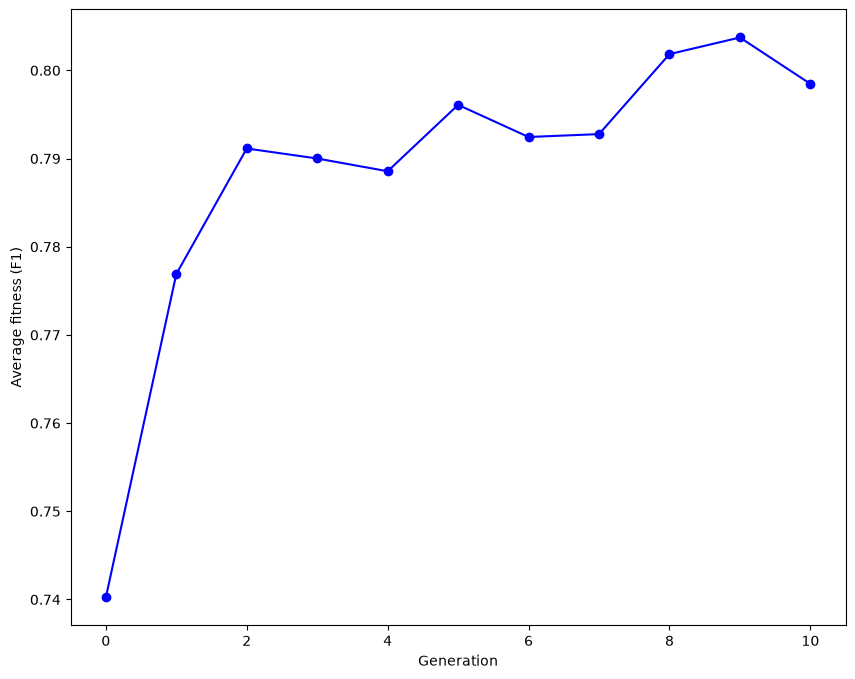
\includegraphics[width=\columnwidth]{avg_fitness}
\caption{Aptitud promedio (F1) de la población por generación.}
\label{fig:avg}
\end{figure}

La población inicial aleatoria ya contenía un individuo con F1 de 0,8066, pero su promedio era bajo (0,7402) y su dispersión alta (0,0822). El valor máximo alcanzó 0,8125 en la tercera generación; sin embargo, en las generaciones 5 y 6 ese individuo se perdió y el máximo retrocedió a 0,8101, para recuperarse en la generación 7 y mantenerse hasta el final. La aptitud promedio creció de 0,7402 a 0,7985, con un pico de 0,8037 en la generación 9. La desviación estándar se redujo con respecto a la población inicial, aunque osciló entre 0,018 y 0,045 debido a la aparición ocasional de individuos de baja aptitud producidos por la mutación.

\subsection{Mejor individuo}
El mejor individuo de la población final fue
\begin{equation*}
\mathbf{x}^{*} = [0,0,0,0,1,0,0,0,0,1,0,0,0,1,1],
\end{equation*}
que selecciona los atributos con índices $\{4, 9, 13, 14\}$, es decir, 4 de los 15 atributos disponibles, con un puntaje F1 de 0,8125. La cardinalidad del subconjunto coincide exactamente con el número de atributos informativos del conjunto de datos.

\section{Discusión}\label{sec:discusion}
Los resultados muestran que el AG converge rápidamente hacia una región de alta aptitud: el mejor valor se alcanzó en la tercera generación y no fue superado en las siete restantes. Esto sugiere que, para un espacio de búsqueda de $2^{15} = 32\,768$ configuraciones, 10 generaciones con 100 individuos (menos de 600 evaluaciones efectivas) son suficientes para localizar un buen subconjunto, aunque no garantizan el óptimo global.

El retroceso del máximo en las generaciones 5 y 6 y la persistencia de individuos con aptitud baja (mínimos entre 0,55 y 0,67) son consecuencia directa del reemplazo generacional sin elitismo combinado con la mutación: el mejor individuo no tiene garantizada su supervivencia y puede perderse o degradarse. Agregar elitismo (conservar los $k$ mejores) o usar un esquema de reemplazo $(\mu + \lambda)$ eliminaría ese retroceso y reduciría la variabilidad.

Cabe señalar que el generador de números aleatorios del AG no se fijó con una semilla, de modo que ejecuciones sucesivas producen trayectorias distintas. En una ejecución previa el mejor individuo seleccionó 5 atributos ($\{0, 4, 9, 13, 14\}$) con F1 de 0,8129, un resultado muy cercano al aquí reportado, lo que sugiere que el método es estable aunque el subconjunto exacto varíe.

Finalmente, la función de aptitud no penaliza el número de atributos seleccionados. Dos individuos con igual F1 pero distinta cardinalidad son indistinguibles para el AG, de modo que la parsimonia del resultado obtenido es fortuita y no una propiedad garantizada del método.

\section{Conclusiones y trabajo futuro}\label{sec:conclusiones}
Se implementó un algoritmo genético simple para selección de características que, con una configuración estándar de operadores y sin ajuste fino de hiperparámetros, redujo el conjunto de 15 a 4 atributos manteniendo un F1 de 0,8125 bajo validación cruzada estratificada. La codificación binaria resultó natural para el problema y la biblioteca DEAP permitió una implementación compacta.

Como trabajo futuro se propone: (i) incorporar elitismo o reemplazo $(\mu+\lambda)$ para evitar la pérdida del mejor individuo; (ii) penalizar la cardinalidad en la función de aptitud o formular el problema como multiobjetivo (F1 frente a número de atributos) usando NSGA-II; (iii) fijar la semilla del generador aleatorio y repetir el experimento con varias semillas para estimar la variabilidad del resultado; y (iv) validar el método sobre conjuntos de datos reales y con clasificadores no lineales, incluyendo redes neuronales.

\begin{thebibliography}{00}
\bibitem{holland1975} J. H. Holland, \emph{Adaptation in Natural and Artificial Systems}. Ann Arbor, MI, USA: University of Michigan Press, 1975.
\bibitem{goldberg1989} D. E. Goldberg, \emph{Genetic Algorithms in Search, Optimization, and Machine Learning}. Reading, MA, USA: Addison-Wesley, 1989.
\bibitem{deap2012} F.-A. Fortin, F.-M. De Rainville, M.-A. Gardner, M. Parizeau y C. Gagné, ``DEAP: Evolutionary algorithms made easy,'' \emph{Journal of Machine Learning Research}, vol. 13, pp. 2171--2175, 2012.
\bibitem{sklearn2011} F. Pedregosa \emph{et al.}, ``Scikit-learn: Machine learning in Python,'' \emph{Journal of Machine Learning Research}, vol. 12, pp. 2825--2830, 2011.
\bibitem{guyon2003} I. Guyon, ``Design of experiments for the NIPS 2003 variable selection benchmark,'' NIPS 2003 Feature Selection Challenge, 2003.
\end{thebibliography}

\end{document}
